% fig05_decel_ladder.tex — AD/ELENA relativistic deceleration ladder T(p).
% Compiled by the paper Makefile via `make figures` (pdflatex on the snippet).
%
% Data: §Method (deceleration) + companion/verify-ledger.json (rel_* atoms).
% T(p) = sqrt((pc)^2 + (m_p c^2)^2) - m_p c^2, with m_p c^2 = 938.272 MeV.
% Registered verify-atom rungs (marked):
%   AD-in : p=3500 MeV/c -> T=2685.31 MeV
%   AD-out: p=100         -> T=5.3139  MeV
%   ELENA : T=0.1         -> p=13.6991 MeV/c
% Log-log so the GeV->keV span (~5 decades in T) is visible.
%
% Manual single-shot compile (debug):
%   pdflatex -interaction=nonstopmode -halt-on-error fig05_decel_ladder.tex
\documentclass[border=4pt]{standalone}
\usepackage{tikz}
\usepackage{pgfplots}
\pgfplotsset{compat=1.18}
\begin{document}
% T(p) = sqrt(p^2 + 938.272^2) - 938.272 ; m_p c^2 = 938.272 MeV
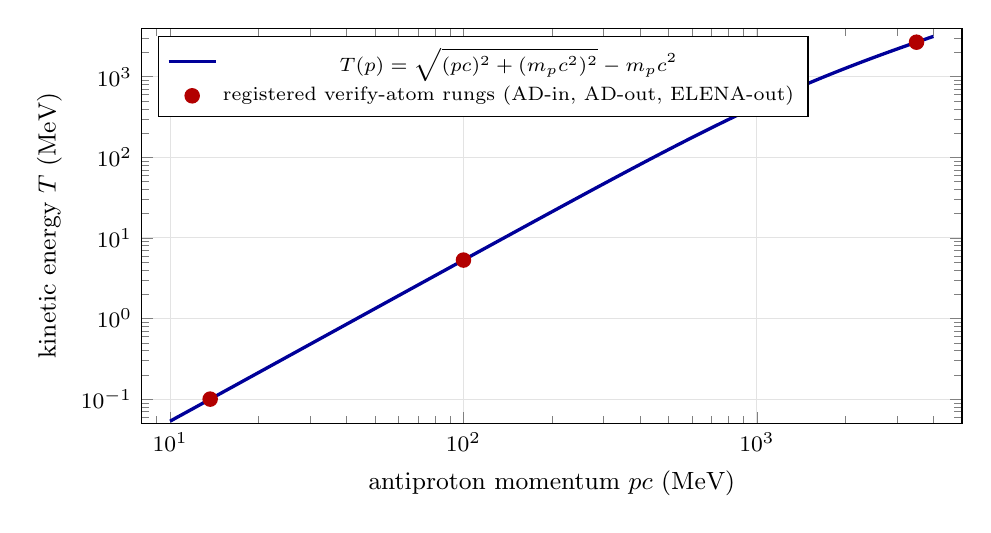
\begin{tikzpicture}
\begin{axis}[
  width=12cm, height=6.6cm,
  xmode=log, ymode=log,
  domain=10:4000, samples=120,
  xlabel={antiproton momentum $pc$ (MeV)},
  ylabel={kinetic energy $T$ (MeV)},
  tick label style={font=\footnotesize},
  label style={font=\small},
  xmin=8, xmax=5000, ymin=0.05, ymax=4000,
  ymajorgrids, xmajorgrids, grid style={gray!22},
  legend style={font=\scriptsize, at={(0.02,0.98)}, anchor=north west},
]
\addplot[blue!60!black, very thick, smooth] {
  sqrt(x^2 + 938.272^2) - 938.272
};
\addlegendentry{$T(p)=\sqrt{(pc)^2+(m_pc^2)^2}-m_pc^2$}
\addplot[only marks, mark=*, mark size=2.6pt, red!70!black] coordinates {
  (3500, 2685.31)
  (100,  5.3139)
  (13.6991, 0.1)
};
\addlegendentry{registered verify-atom rungs (AD-in, AD-out, ELENA-out)}
\end{axis}
\end{tikzpicture}
\end{document}
